\begin{pastexam}[label={px:gk3-112-ds-04}]{高考三級資訊處理 112 年 第四題}
（申論；25 分）

某一系統有下表所示的使用者帳號與密碼資料，今為了保密需要欲將使用者密碼透過雜湊函數加以加密，並將雜湊後的密碼連同使用者帳號儲存於一個2-3樹（2-3 tree）（依使用者帳號英文字母順序儲存），而雜湊函數$\mathrm{h}(\mathrm{x})=$密碼之英文及數字加總，其中英文a-z相當於1-26。
\begin{center}
\renewcommand{\arraystretch}{1.2}
\begin{tabular}{|c|c|}
\hline
\makebox[6em]{使用者帳號} & \makebox[6em]{使用者密碼} \\ \hline
AA & 234abc \\ \hline
BB & 123bcd \\ \hline
CD & aa012 \\ \hline
AC & 555be \\ \hline
BD & 45fdd \\ \hline
CA & 712ccc \\ \hline
\end{tabular}
\end{center}
\begin{itemize}[leftmargin=2.2em]
\item[㈠] 試計算出雜湊後的密碼資料。（10分）
\item[㈡] 試建立此2-3樹，以儲存系統的使用者帳號與（雜湊後）密碼資料。（15分）
\end{itemize}
\end{pastexam}

\begin{pastsoln}
答案：㈠ AA $\to 15$、BB $\to 15$、CD $\to 5$、AC $\to 22$、BD $\to 23$、CA $\to 19$；㈡ 根是 $[\mathrm{BB}, \mathrm{CA}]$，
三個葉節點 $[\mathrm{AA}, \mathrm{AC}]$、$[\mathrm{BD}]$、$[\mathrm{CD}]$。

\textbf{㈠}。 「英文及數字加總」理解成每個數字字元取它的值、每個英文字母取 a $= 1$、b $= 2$、……、z $= 26$，全部
相加（不是把 234 當成兩百三十四）。
\begin{center}
\begin{tabular}{lll}
\toprule
帳號 & 密碼 & $h$ \\
\midrule
AA & 234abc & $2 + 3 + 4 + 1 + 2 + 3 = 15$ \\
BB & 123bcd & $1 + 2 + 3 + 2 + 3 + 4 = 15$ \\
CD & aa012 & $1 + 1 + 0 + 1 + 2 = 5$ \\
AC & 555be & $5 + 5 + 5 + 2 + 5 = 22$ \\
BD & 45fdd & $4 + 5 + 6 + 4 + 4 = 23$ \\
CA & 712ccc & $7 + 1 + 2 + 3 + 3 + 3 = 19$ \\
\bottomrule
\end{tabular}
\end{center}
AA 和 BB 的雜湊值相同（都是 $15$），這個雜湊函數碰撞很容易發生；不過 2-3 樹是用帳號排序，雜湊值只是附帶存的
資料，碰撞不影響建樹。 （題目說「加密」，其實雜湊不是加密，也不能還原；拿來存密碼時，登入是把輸入的密碼雜湊後
和存的值比對。 這麼簡單的雜湊函數實務上不安全。）

\textbf{㈡}。 依表的順序，以帳號（字母順序 AA $<$ AC $<$ BB $<$ BD $<$ CA $<$ CD）為鍵插入 2-3 樹，每個鍵附帶雜湊值。
2-3 樹的插入（資結書第~11.1.3~節）：找到該放的葉節點放進去，若變成 $3$ 個鍵就把中間的鍵往上送、左右分成兩個節點；
父節點因此變成 $3$ 個鍵時繼續往上分裂。 下面節點裡只寫帳號，雜湊值跟著帳號走。
\begin{center}
\small
\begin{tabular}{lll}
\toprule
插入 & 過程 & 插入後的樹 \\
\midrule
AA & 空樹，成為根 & $[\mathrm{AA}]$ \\
BB & 放進根 & $[\mathrm{AA}, \mathrm{BB}]$ \\
CD & 根變成 $[\mathrm{AA}, \mathrm{BB}, \mathrm{CD}]$，分裂，BB 上升成新根 & $[\mathrm{BB}]$；$[\mathrm{AA}]$、$[\mathrm{CD}]$ \\
AC & AC $<$ BB，放進左葉 & $[\mathrm{BB}]$；$[\mathrm{AA}, \mathrm{AC}]$、$[\mathrm{CD}]$ \\
BD & BD $>$ BB，放進右葉 & $[\mathrm{BB}]$；$[\mathrm{AA}, \mathrm{AC}]$、$[\mathrm{BD}, \mathrm{CD}]$ \\
CA & 右葉變成 $[\mathrm{BD}, \mathrm{CA}, \mathrm{CD}]$，分裂，CA 上升到根 & $[\mathrm{BB}, \mathrm{CA}]$；$[\mathrm{AA}, \mathrm{AC}]$、$[\mathrm{BD}]$、$[\mathrm{CD}]$ \\
\bottomrule
\end{tabular}
\end{center}
最後的 2-3 樹（每格是「帳號：雜湊後密碼」）：
\begin{center}
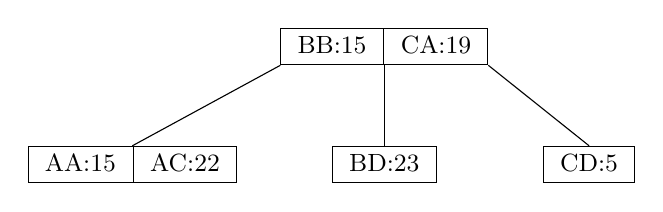
\begin{tikzpicture}[k/.style={draw,inner sep=0pt,font=\small}]
\node[k] (r) at (0,0) {\begin{tabular}{c|c}BB:15 & CA:19\end{tabular}};
\node[k] (a) at (-3.2,-1.5) {\begin{tabular}{c|c}AA:15 & AC:22\end{tabular}};
\node[k] (b) at (0,-1.5) {\begin{tabular}{c}BD:23\end{tabular}};
\node[k] (c) at (2.6,-1.5) {\begin{tabular}{c}CD:5\end{tabular}};
\draw (r.south west) -- (a.north);
\draw (r.south) -- (b.north);
\draw (r.south east) -- (c.north);
\end{tikzpicture}
\end{center}
檢查：每個葉節點都在同一層；根有 $2$ 個鍵、$3$ 個子節點；左子樹的帳號都 $<$ BB，中間的介於 BB 和 CA 之間，右邊的都 $>$ CA，
是合法的 2-3 樹。 中序走訪得到 AA, AC, BB, BD, CA, CD，正是字母順序。 若題目的意思是依帳號的字母順序
（AA, AC, BB, BD, CA, CD）插入，結果會不同：依序插入後是根 $[\mathrm{AC}, \mathrm{BD}]$、葉 $[\mathrm{AA}]$、$[\mathrm{BB}]$、
$[\mathrm{CA}, \mathrm{CD}]$；本書照表格的順序插入。
\end{pastsoln}
